\documentclass[12pt,a4paper]{report}

\usepackage[margin=1in]{geometry}
\usepackage{graphicx}
\usepackage{amsmath}
\usepackage{booktabs}
\usepackage{array}
\usepackage{longtable}
\usepackage{float}
\usepackage{enumitem}
\usepackage{listings}
\usepackage{xcolor}
\usepackage{setspace}
\usepackage{titlesec}
\usepackage[hidelinks]{hyperref}
\usepackage{tikz}
\usetikzlibrary{shapes.geometric,arrows.meta,positioning,fit,calc}

\setstretch{1.15}

\lstset{
  basicstyle=\ttfamily\small,
  frame=single,
  breaklines=true,
  backgroundcolor=\color{gray!8},
  showstringspaces=false
}

% ---------- TikZ styles ----------
\tikzset{
  box/.style={rectangle, draw, rounded corners=3pt, minimum height=0.9cm,
              minimum width=2.4cm, align=center, font=\small, fill=blue!8},
  dbox/.style={rectangle, draw, rounded corners=3pt, minimum height=0.9cm,
              minimum width=2.4cm, align=center, font=\small, fill=green!10},
  dec/.style={diamond, draw, aspect=2.5, align=center, font=\small, fill=yellow!15,
              inner sep=1pt},
  uc/.style={ellipse, draw, align=center, font=\footnotesize, fill=orange!10,
             minimum height=0.8cm},
  cls/.style={rectangle, draw, align=left, font=\scriptsize, fill=blue!6,
              minimum width=2.6cm},
  arr/.style={-{Latex[length=2.2mm]}, thick}
}

\begin{document}

% =====================================================
% TITLE PAGE
% =====================================================
\begin{titlepage}
\centering
{\Large \textbf{THAPAR INSTITUTE OF ENGINEERING AND TECHNOLOGY}\par}
\vspace{0.3cm}
{\large PATIALA, PUNJAB\par}
\vspace{0.8cm}
{\large \textbf{DEPARTMENT OF COMPUTER SCIENCE AND ENGINEERING}\par}
\vspace{2cm}
{\Huge \textbf{CodeShield}\par}
\vspace{0.5cm}
{\LARGE ML-Based Code Vulnerability Detection and Risk Assessment Platform\par}
\vspace{1cm}
{\Large \textbf{Evaluation Report}\par}
\vspace{2cm}
{\large Submitted to: \textbf{Ms. Paramveer Kaur}\par}
{\large Course: UCS503\par}
{\large Degree: B.E. Computer Engineering\par}
\vspace{1.5cm}
{\large \textbf{Team Members}\par}
\vspace{0.3cm}
\begin{tabular}{ll}
Rhea Balamurugan & 1024030152\\
Ishi Govil & 1024030161\\
Shreya Kush & 1024030718
\end{tabular}
\vfill
{\large 2026\par}
\end{titlepage}

\pagenumbering{roman}
\tableofcontents
\clearpage
\pagenumbering{arabic}

% =====================================================
% CHAPTER 1
% =====================================================
\chapter{Introduction}

\section{Background and Context}
Modern software systems contain large volumes of source code and may contain security weaknesses that are difficult to identify through manual inspection alone. Vulnerabilities can remain hidden during normal execution and may only become visible after exploitation.

CodeShield is a software-security platform that combines static code analysis with machine learning. The system accepts source code, analyzes it, identifies selected vulnerability categories, estimates risk, and presents the findings through a developer-facing dashboard. The project aims to identify selected vulnerabilities rather than claim exhaustive detection of every possible weakness.

\section{Problem Statement}
CodeShield addresses the following problems:
\begin{itemize}[noitemsep]
  \item Large codebases are difficult to inspect manually.
  \item Security vulnerabilities may not produce visible runtime errors, and fixing them after deployment is costly.
  \item Different vulnerability classes require different detection strategies.
  \item Developers need prioritization so that critical findings can be addressed first.
\end{itemize}

\section{Project Objectives}
\begin{enumerate}[noitemsep]
  \item Develop a web-based interface for submitting source code.
  \item Build a FastAPI backend that manages scan requests and analysis.
  \item Combine static-analysis rules and machine-learning predictions to detect vulnerabilities.
  \item Provide vulnerability type, severity, confidence, location, and explanation.
  \item Store results and present them through a dashboard.
  \item Evaluate the system using both ML and software-system metrics.
\end{enumerate}

\section{Scope}
The project currently focuses on the following vulnerability categories:
\begin{itemize}[noitemsep]
  \item SQL Injection
  \item Command Injection
  \item Hardcoded Credentials
  \item Cross-Site Scripting (XSS)
  \item Insecure File Handling
\end{itemize}
The ML model works on Python code. Additional languages and vulnerability classes can be incorporated as future extensions.

% =====================================================
% CHAPTER 2
% =====================================================
\chapter{Software Development Life Cycle and Project Process}

\section{Selected SDLC Model}
For CodeShield, an iterative and incremental approach is followed. The project has several components---frontend, backend, database, static analysis, ML pipeline, risk assessment and reporting---that can be developed, tested and integrated step by step.

\section{SDLC Diagram}
\begin{figure}[H]
\centering
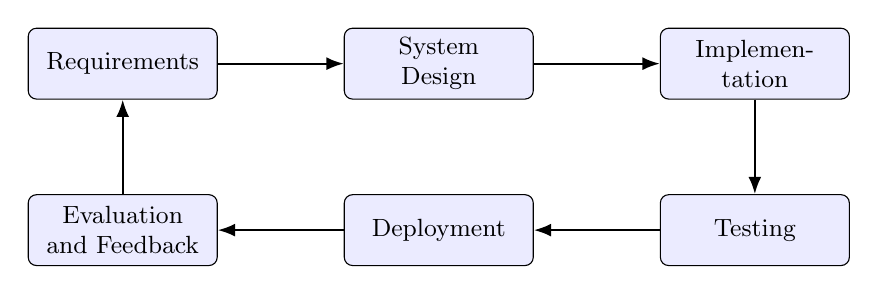
\begin{tikzpicture}[node distance=1.6cm]
  \node[box] (r) {Requirements};
  \node[box, right=of r] (d) {System\\Design};
  \node[box, right=of d] (i) {Implemen-\\tation};
  \node[box, below=1.2cm of i] (t) {Testing};
  \node[box, left=of t] (dp) {Deployment};
  \node[box, left=of dp] (e) {Evaluation\\and Feedback};
  \draw[arr] (r)--(d);
  \draw[arr] (d)--(i);
  \draw[arr] (i)--(t);
  \draw[arr] (t)--(dp);
  \draw[arr] (dp)--(e);
  \draw[arr] (e) -- (r);
\end{tikzpicture}
\caption{Iterative and incremental SDLC adopted for CodeShield.}
\end{figure}

\section{Development Increments}
\begin{enumerate}[noitemsep]
  \item \textbf{Increment 1:} Requirements, architecture and UI design.
  \item \textbf{Increment 2:} React frontend and FastAPI backend.
  \item \textbf{Increment 3:} Source-code parsing and static-analysis rules.
  \item \textbf{Increment 4:} Dataset preparation and ML model development.
  \item \textbf{Increment 5:} ML--backend integration and risk assessment.
  \item \textbf{Increment 6:} Testing, evaluation and dashboard refinement.
\end{enumerate}

% =====================================================
% CHAPTER 3
% =====================================================
\chapter{Requirements Analysis}

\section{Functional Requirements}
\begin{longtable}{p{1.2cm}p{13cm}}
\toprule
\textbf{ID} & \textbf{Requirement}\\
\midrule
\endhead
FR1 & The system shall allow a developer to submit source code.\\
FR2 & The system shall preprocess and parse the submitted source code.\\
FR3 & The system shall perform static-analysis checks.\\
FR4 & The system shall apply the trained ML model to supported code.\\
FR5 & The system shall identify supported vulnerability categories.\\
FR6 & The system shall generate severity and confidence information.\\
FR7 & The system shall report affected file and line information when available.\\
FR8 & The system shall store scan information in the database.\\
FR9 & The system shall display scan results through the dashboard.\\
\bottomrule
\end{longtable}

\section{Non-Functional Requirements}
\begin{itemize}[noitemsep]
  \item \textbf{Performance:} Scans should complete within a practical time for the supported input size.
  \item \textbf{Reliability:} Invalid code and failed scans should be handled gracefully.
  \item \textbf{Security:} Submitted code should be processed with controlled access.
  \item \textbf{Maintainability:} Static-analysis rules and ML models should be modular.
  \item \textbf{Usability:} Results should be understandable to developers.
\end{itemize}

% =====================================================
% CHAPTER 4
% =====================================================
\chapter{System Architecture and Design}

\section{Use Case Diagram}
The primary actor is the Developer, who submits code, starts a scan, and views results. The system internally performs preprocessing, static analysis, ML analysis, risk assessment and report generation.

\begin{figure}[H]
\centering
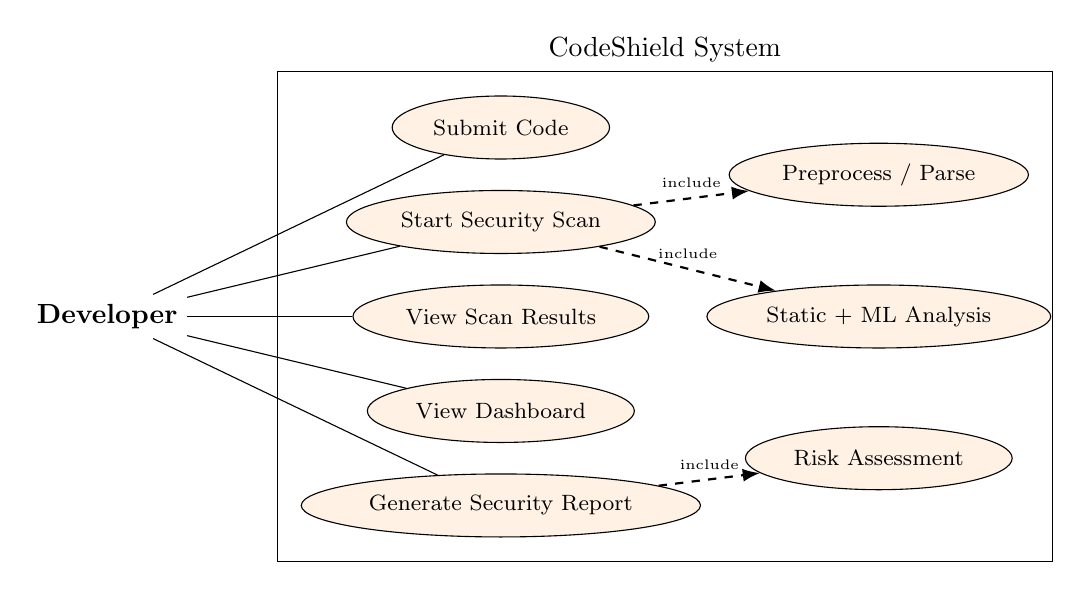
\begin{tikzpicture}[node distance=0.6cm]
  \node (dev) at (0,0) {\textbf{Developer}};
  \node[uc] (u1) at (5,2.4) {Submit Code};
  \node[uc] (u2) at (5,1.2) {Start Security Scan};
  \node[uc] (u3) at (5,0) {View Scan Results};
  \node[uc] (u4) at (5,-1.2) {View Dashboard};
  \node[uc] (u5) at (5,-2.4) {Generate Security Report};
  \node[uc] (i1) at (9.8,1.8) {Preprocess / Parse};
  \node[uc] (i2) at (9.8,0) {Static + ML Analysis};
  \node[uc] (i3) at (9.8,-1.8) {Risk Assessment};
  \foreach \u in {u1,u2,u3,u4,u5} \draw (dev) -- (\u);
  \draw[arr, dashed] (u2) -- node[above,font=\tiny]{include} (i1);
  \draw[arr, dashed] (u2) -- node[above,font=\tiny]{include} (i2);
  \draw[arr, dashed] (u5) -- node[above,font=\tiny]{include} (i3);
  \node[draw, fit=(u1)(u5)(i1)(i3), inner sep=0.3cm, label=above:{CodeShield System}] {};
\end{tikzpicture}
\caption{Use case diagram for CodeShield.}
\end{figure}

\section{High-Level System Architecture}
The React frontend sends the code to the FastAPI backend, which connects to the analysis pipeline. The pipeline performs code parsing, static analysis and ML-based analysis, followed by result fusion, risk assessment and reporting. Results are stored in PostgreSQL.

\begin{figure}[H]
\centering
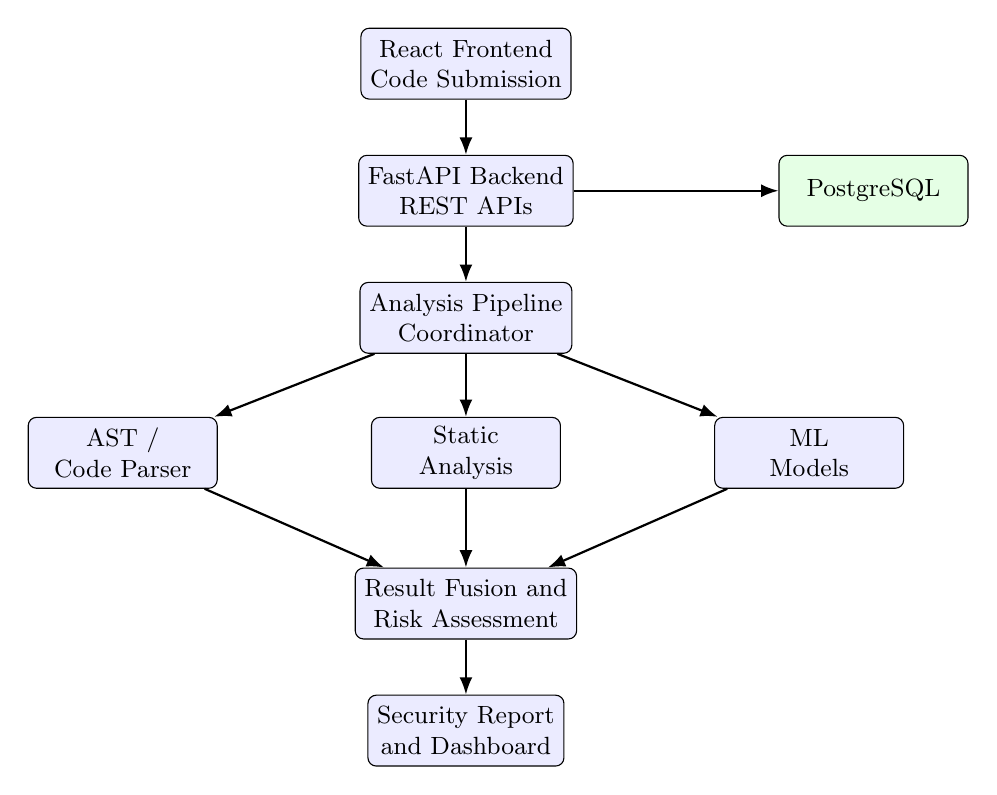
\begin{tikzpicture}[node distance=0.7cm]
  \node[box] (fe) {React Frontend\\Code Submission};
  \node[box, below=of fe] (be) {FastAPI Backend\\REST APIs};
  \node[box, below=of be] (ap) {Analysis Pipeline\\Coordinator};
  \node[box, below left=0.8cm and 0.3cm of ap, xshift=-1.5cm] (ast) {AST /\\Code Parser};
  \node[box, below=0.8cm of ap] (sa) {Static\\Analysis};
  \node[box, below right=0.8cm and 0.3cm of ap, xshift=1.5cm] (ml) {ML\\Models};
  \node[box, below=1.0cm of sa] (fu) {Result Fusion and\\Risk Assessment};
  \node[box, below=of fu] (rep) {Security Report\\and Dashboard};
  \node[dbox, right=2.6cm of be] (db) {PostgreSQL};
  \draw[arr] (fe)--(be);
  \draw[arr] (be)--(ap);
  \draw[arr] (ap)--(ast);
  \draw[arr] (ap)--(sa);
  \draw[arr] (ap)--(ml);
  \draw[arr] (ast)--(fu);
  \draw[arr] (sa)--(fu);
  \draw[arr] (ml)--(fu);
  \draw[arr] (fu)--(rep);
  \draw[arr] (be)--(db);
\end{tikzpicture}
\caption{End-to-end CodeShield system architecture.}
\end{figure}

\section{Core Scanning Workflow}
\begin{figure}[H]
\centering
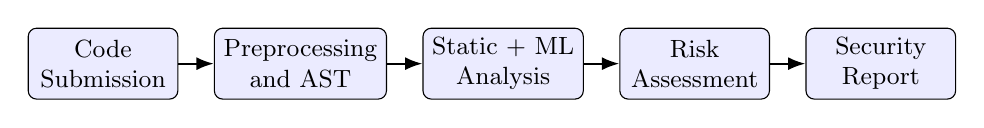
\begin{tikzpicture}[node distance=0.45cm]
  \node[box, minimum width=1.9cm] (a) {Code\\Submission};
  \node[box, minimum width=1.9cm, right=of a] (b) {Preprocessing\\and AST};
  \node[box, minimum width=1.9cm, right=of b] (c) {Static + ML\\Analysis};
  \node[box, minimum width=1.9cm, right=of c] (d) {Risk\\Assessment};
  \node[box, minimum width=1.9cm, right=of d] (e) {Security\\Report};
  \draw[arr] (a)--(b); \draw[arr] (b)--(c); \draw[arr] (c)--(d); \draw[arr] (d)--(e);
\end{tikzpicture}
\caption{CodeShield core vulnerability-scanning workflow.}
\end{figure}

\clearpage
\section{UML Class Diagram}
\begin{figure}[H]
\centering
\begin{tikzpicture}[scale=0.85, transform shape, node distance=0.8cm]
  \node[cls] (dev) {\textbf{Developer}\\\hrule developer\_id\\ name\\ email\\\hrule submitCode()\\ viewDashboard()};
  \node[cls, right=of dev] (scan) {\textbf{Scan}\\\hrule scan\_id\\ created\_at\\ status\\\hrule startScan()\\ getStatus()};
  \node[cls, right=of scan] (src) {\textbf{SourceCode}\\\hrule source\_id\\ file\_name\\ language\\ content\\\hrule parse()\\ validate()};
  \node[cls, below=1.2cm of scan] (ar) {\textbf{AnalysisResult}\\\hrule result\_id\\ method\\ confidence\\ prediction\\\hrule analyze()};
  \node[cls, left=of ar] (rep) {\textbf{SecurityReport}\\\hrule report\_id\\ created\_at\\ summary\\\hrule generate()\\ export()};
  \node[cls, right=of ar] (vul) {\textbf{Vulnerability}\\\hrule vulnerability\_id\\ type\\ severity\\ line\_number\\ explanation\\\hrule getSeverity()};
  \draw (dev)--(scan);
  \draw (scan)--(src);
  \draw (scan)--(ar);
  \draw (scan)--(rep);
  \draw (ar)--(vul);
\end{tikzpicture}
\caption{UML class diagram for the logical CodeShield software model.}
\end{figure}

\section{Activity Diagram}
\begin{figure}[H]
\centering
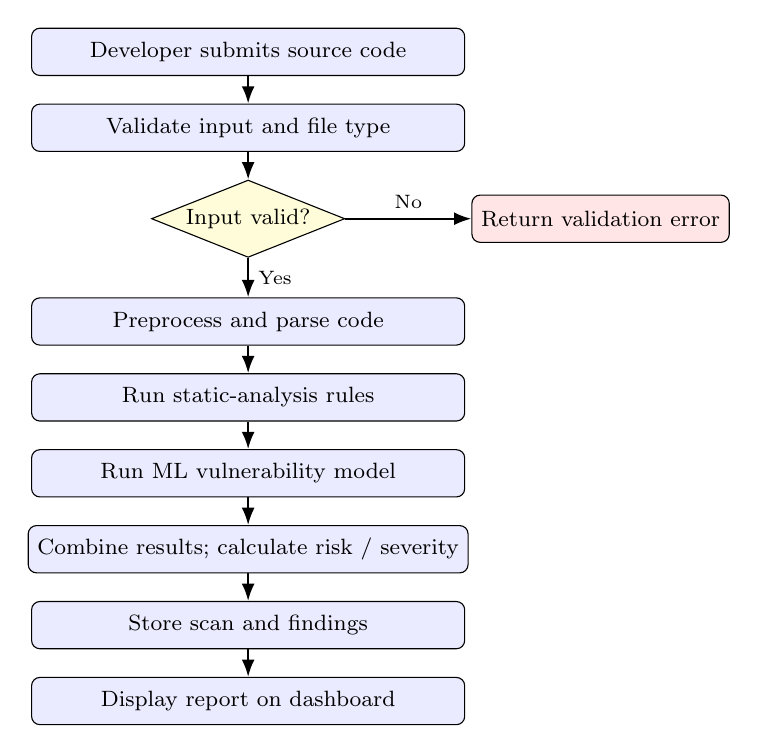
\begin{tikzpicture}[node distance=0.35cm,
  box/.append style={minimum height=0.6cm, font=\footnotesize},
  dec/.append style={font=\footnotesize}]
  \node[box, minimum width=5.5cm] (a) {Developer submits source code};
  \node[box, minimum width=5.5cm, below=of a] (b) {Validate input and file type};
  \node[dec, below=of b] (c) {Input valid?};
  \node[box, right=1.6cm of c, fill=red!10, minimum width=3cm] (err) {Return validation error};
  \node[box, minimum width=5.5cm, below=0.5cm of c] (d) {Preprocess and parse code};
  \node[box, minimum width=5.5cm, below=of d] (e) {Run static-analysis rules};
  \node[box, minimum width=5.5cm, below=of e] (f) {Run ML vulnerability model};
  \node[box, minimum width=5.5cm, below=of f] (g) {Combine results; calculate risk / severity};
  \node[box, minimum width=5.5cm, below=of g] (h) {Store scan and findings};
  \node[box, minimum width=5.5cm, below=of h] (i) {Display report on dashboard};
  \draw[arr] (a)--(b); \draw[arr] (b)--(c);
  \draw[arr] (c)--node[above,font=\scriptsize]{No}(err);
  \draw[arr] (c)--node[right,font=\scriptsize]{Yes}(d);
  \draw[arr] (d)--(e); \draw[arr] (e)--(f); \draw[arr] (f)--(g);
  \draw[arr] (g)--(h); \draw[arr] (h)--(i);
\end{tikzpicture}
\caption{Activity diagram for a CodeShield security scan.}
\end{figure}

% =====================================================
% CHAPTER 5
% =====================================================
\chapter{Methodology and Design}

\section{Code Preprocessing}
The submitted source code is first parsed to extract useful structures depending on the supported language, such as function calls, user-controlled input, database operations, file-system operations and command execution.

\section{Static Analysis}
Static analysis provides a deterministic layer based on predefined security rules. It identifies suspicious patterns without executing the program. For example:
\begin{lstlisting}[language=Python]
query = "SELECT * FROM users WHERE id=" + user_id
\end{lstlisting}
A rule can identify direct concatenation of user-controlled data into an SQL query and generate a potential SQL-injection finding.

\section{Machine Learning Pipeline}
Along with static analysis, the ML pipeline predicts the vulnerability type of a Python code snippet:

\begin{center}
\textit{Python Code $\rightarrow$ TF-IDF $\rightarrow$ Linear SVM $\rightarrow$ Probability Calibration $\rightarrow$ Vulnerability Class + Confidence}
\end{center}

\subsection{TF-IDF Feature Extraction}
The code is treated as text and converted into numerical features using TF-IDF with word-level features, unigrams and bigrams (\texttt{ngram\_range=(1,2)}) and L2 normalization.

\subsection{Linear SVM Classifier}
The classifier is a Linear Support Vector Machine (\texttt{LinearSVC}) with \texttt{class\_weight=balanced} to handle class imbalance and regularization parameter $C=2.0$. It is well suited to high-dimensional sparse TF-IDF features.

\subsection{Probability Calibration and Confidence}
\texttt{LinearSVC} produces decision scores rather than probabilities, so the classifier is wrapped with sigmoid probability calibration. During inference, the backend uses the calibrated \texttt{predict\_proba()} output to select the highest-probability class and return its confidence.

\begin{figure}[H]
\centering
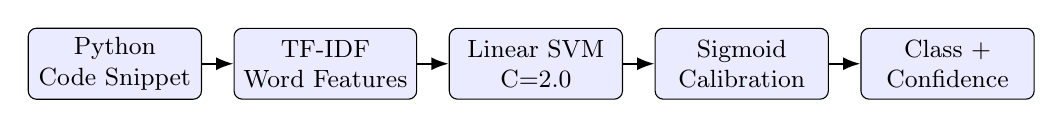
\begin{tikzpicture}[node distance=0.4cm]
  \node[box, minimum width=2.2cm] (a) {Python\\Code Snippet};
  \node[box, minimum width=2.2cm, right=of a] (b) {TF-IDF\\Word Features};
  \node[box, minimum width=2.2cm, right=of b] (c) {Linear SVM\\C=2.0};
  \node[box, minimum width=2.2cm, right=of c] (d) {Sigmoid\\Calibration};
  \node[box, minimum width=2.2cm, right=of d] (e) {Class +\\Confidence};
  \draw[arr] (a)--(b); \draw[arr] (b)--(c); \draw[arr] (c)--(d); \draw[arr] (d)--(e);
\end{tikzpicture}
\caption{Current CodeShield multiclass ML inference pipeline.}
\end{figure}

\section{Vulnerability Information and Risk Assessment}
For every detected vulnerability, CodeShield records its type, severity, confidence, affected location and explanation. Findings are prioritized so that critical issues can be addressed first.

\section{Result Fusion}
Static-analysis findings and ML predictions are combined into a unified set of findings, which is then passed to risk assessment and reporting.

% =====================================================
% CHAPTER 6
% =====================================================
\chapter{Implementation}

\section{Frontend}
The frontend is developed using React for code submission and for displaying vulnerability results through the dashboard.

\section{Backend}
The backend is implemented using Python and FastAPI. It manages scan requests, validates input, and connects the frontend with the analysis pipeline.
\begin{lstlisting}
Frontend -> FastAPI -> Validation -> Analysis (Rules + ML)
         -> Risk Assessment -> Database -> Response
\end{lstlisting}
A health endpoint \texttt{GET /health} verifies that the service is running.

\section{Database}
PostgreSQL is used for persistent storage. The logical entities are Developer/User, Scan, Source Code, Vulnerability, Analysis Result and Security Report.

\section{ML Model Integration}
The trained model is integrated with the FastAPI backend so that predictions are generated during the scanning process. It applies the same TF-IDF transformation used in training, passes the features to the calibrated Linear SVM, and returns the predicted class with its calibrated confidence. This output is fused with the static-analysis findings and passed to risk assessment.

% =====================================================
% CHAPTER 7
% =====================================================
\chapter{Testing and Evaluation}

\section{Testing Methodology}
The system was tested at both the software-system and ML levels.
\begin{itemize}[noitemsep]
  \item \textbf{Unit testing:} preprocessing, parsing, static rules, ML prediction, risk scoring and API endpoints.
  \item \textbf{Integration testing:} frontend $\rightarrow$ backend, backend $\rightarrow$ pipeline, pipeline $\rightarrow$ ML model, pipeline $\rightarrow$ PostgreSQL.
  \item \textbf{System testing:} complete scans on safe and known-vulnerable examples.
  \item \textbf{ML testing:} accuracy, precision, recall, F1-score and confusion matrix.
\end{itemize}

\section{Performance Metrics}
ML evaluation uses accuracy, precision, recall, F1-score and the confusion matrix. System-level evaluation includes scanning time and API response time.

\section{Results Table}
System-level values must be measured from the deployed backend and are therefore not fabricated here.

\begin{table}[H]
\centering
\caption{CodeShield evaluation results currently available.}
\begin{tabular}{ll}
\toprule
\textbf{Metric} & \textbf{Achieved}\\
\midrule
Accuracy & 90.00\%\\
Macro F1-score & 91.81\%\\
Weighted F1-score & 90.00\%\\
Test samples & 60\\
Average Scan Time & To be measured\\
API Response Time & To be measured\\
\bottomrule
\end{tabular}
\end{table}

An accuracy of 90\% corresponds to about 54 correctly classified snippets out of 60. Macro F1 gives equal importance to each vulnerability class, which is useful for an imbalanced dataset.

\section{Model Configuration}
\begin{table}[H]
\centering
\caption{Configuration of the current CodeShield ML classifier.}
\begin{tabular}{ll}
\toprule
\textbf{Component} & \textbf{Configuration}\\
\midrule
Input & Python source-code snippet\\
Feature extraction & TF-IDF (word-level)\\
N-grams & Unigrams + bigrams\\
Normalization & L2\\
Classifier & LinearSVC, balanced class weights, $C=2.0$\\
Calibration & Sigmoid probability calibration\\
Output & Vulnerability class + confidence\\
\bottomrule
\end{tabular}
\end{table}

\section{Confusion Matrix}
The confusion matrix values are yet to be added from the final test run. They should be inserted from the same 60-sample run rather than estimated from aggregate metrics.

\begin{figure}[H]
\centering
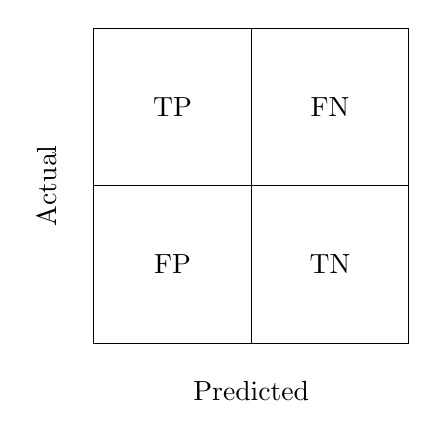
\begin{tikzpicture}
  \draw (0,0) rectangle (2,2);
  \draw (2,0) rectangle (4,2);
  \draw (0,-2) rectangle (2,0);
  \draw (2,-2) rectangle (4,0);
  \node at (1,1) {TP}; \node at (3,1) {FN};
  \node at (1,-1) {FP}; \node at (3,-1) {TN};
  \node[rotate=90] at (-0.6,0) {Actual};
  \node at (2,-2.6) {Predicted};
\end{tikzpicture}
\caption{Confusion matrix layout; replace the cells with measured values from the final test run.}
\end{figure}

% =====================================================
% CHAPTER 8
% =====================================================
\chapter{Results and Analysis}

\section{Example Vulnerability Detection}
Consider the vulnerable query construction:
\begin{lstlisting}[language=Python]
query = "SELECT * FROM users WHERE id=" + user_id
\end{lstlisting}
CodeShield reports the vulnerability type, severity, location, confidence and the reason the code is considered unsafe.

\begin{table}[H]
\centering
\caption{Illustrative CodeShield vulnerability report.}
\begin{tabular}{lp{8cm}}
\toprule
\textbf{Field} & \textbf{Example Result}\\
\midrule
Vulnerability & SQL Injection\\
Severity & High\\
Confidence & Model-generated calibrated probability\\
File & database.py\\
Line & 12\\
Explanation & User-controlled input is concatenated into SQL\\
\bottomrule
\end{tabular}
\end{table}

\section{Challenges and Mitigation}
\begin{table}[H]
\centering
\caption{Major challenges and mitigation strategies.}
\begin{tabular}{p{4cm}p{9.5cm}}
\toprule
\textbf{Challenge} & \textbf{Mitigation}\\
\midrule
False positives & Combine ML predictions with static-analysis rules and confidence scores.\\
False negatives & Measure recall and clearly define supported vulnerability categories.\\
Limited labelled data & Use validated vulnerability datasets and controlled examples.\\
\bottomrule
\end{tabular}
\end{table}

% =====================================================
% CHAPTER 9
% =====================================================
\chapter{Conclusion and Future Work}

\section{Summary of Work}
CodeShield combines static analysis and machine learning to detect selected source-code vulnerabilities. The platform integrates a React frontend, a FastAPI backend, PostgreSQL storage, and an analysis pipeline containing parsing, static rules, ML classification, risk assessment and reporting.

\section{Key Findings}
The calibrated TF-IDF + Linear SVM model achieved 90\% accuracy and a 91.81\% macro F1-score on 60 test samples. Static analysis contributes deterministic findings, while the ML model adds data-driven classification with a confidence score.

\section{Future Work}
\begin{enumerate}[noitemsep]
  \item GitHub repository scanning.
  \item Support for additional programming languages.
  \item Improved ML models.
  \item Better severity prioritization.
  \item Automated remediation suggestions.
  \item Scan history, asynchronous scanning and Docker-based isolated analysis.
\end{enumerate}

\section{Final Remarks}
The project shows that conventional static analysis and machine learning can be combined rather than treated as competing approaches, helping developers identify and prioritize security weaknesses earlier in the development lifecycle.

% =====================================================
% BIBLIOGRAPHY
% =====================================================
\begin{thebibliography}{9}
\bibitem{nist} National Institute of Standards and Technology, \textit{Software Assurance Metrics and Tool Evaluation}, NIST.
\bibitem{owasp} OWASP Foundation, \textit{OWASP Benchmark Project}, OWASP.
\bibitem{bigvul} K. Chhabra et al., \textit{Big-Vul: A Large-Scale Vulnerability Dataset}, GitHub repository and associated research resources.
\bibitem{juliet} National Institute of Standards and Technology, \textit{Juliet Test Suite}, Software Assurance Reference Dataset.
\bibitem{fastapi} FastAPI Documentation, \textit{FastAPI: Modern, Fast Web Framework for Building APIs with Python}.
\bibitem{react} React Documentation, \textit{React: The library for web and native user interfaces}.
\end{thebibliography}

\end{document}
